\documentclass{article}

\usepackage{graphicx}
\usepackage{tikz}
\usepackage{tikzsymbols}
\usetikzlibrary{calc,patterns,shapes.geometric}
\pagestyle{empty}
\usepackage[margin=0pt]{geometry}
\geometry{papersize={14in,12in}}

\def\centerarc[#1](#2)(#3:#4:#5){\draw[#1] ($(#2)+({#5*cos(#3)},{#5*sin(#3)})$) arc (#3:#4:#5);}

\begin{document}
	\begin{figure}
		\centering
		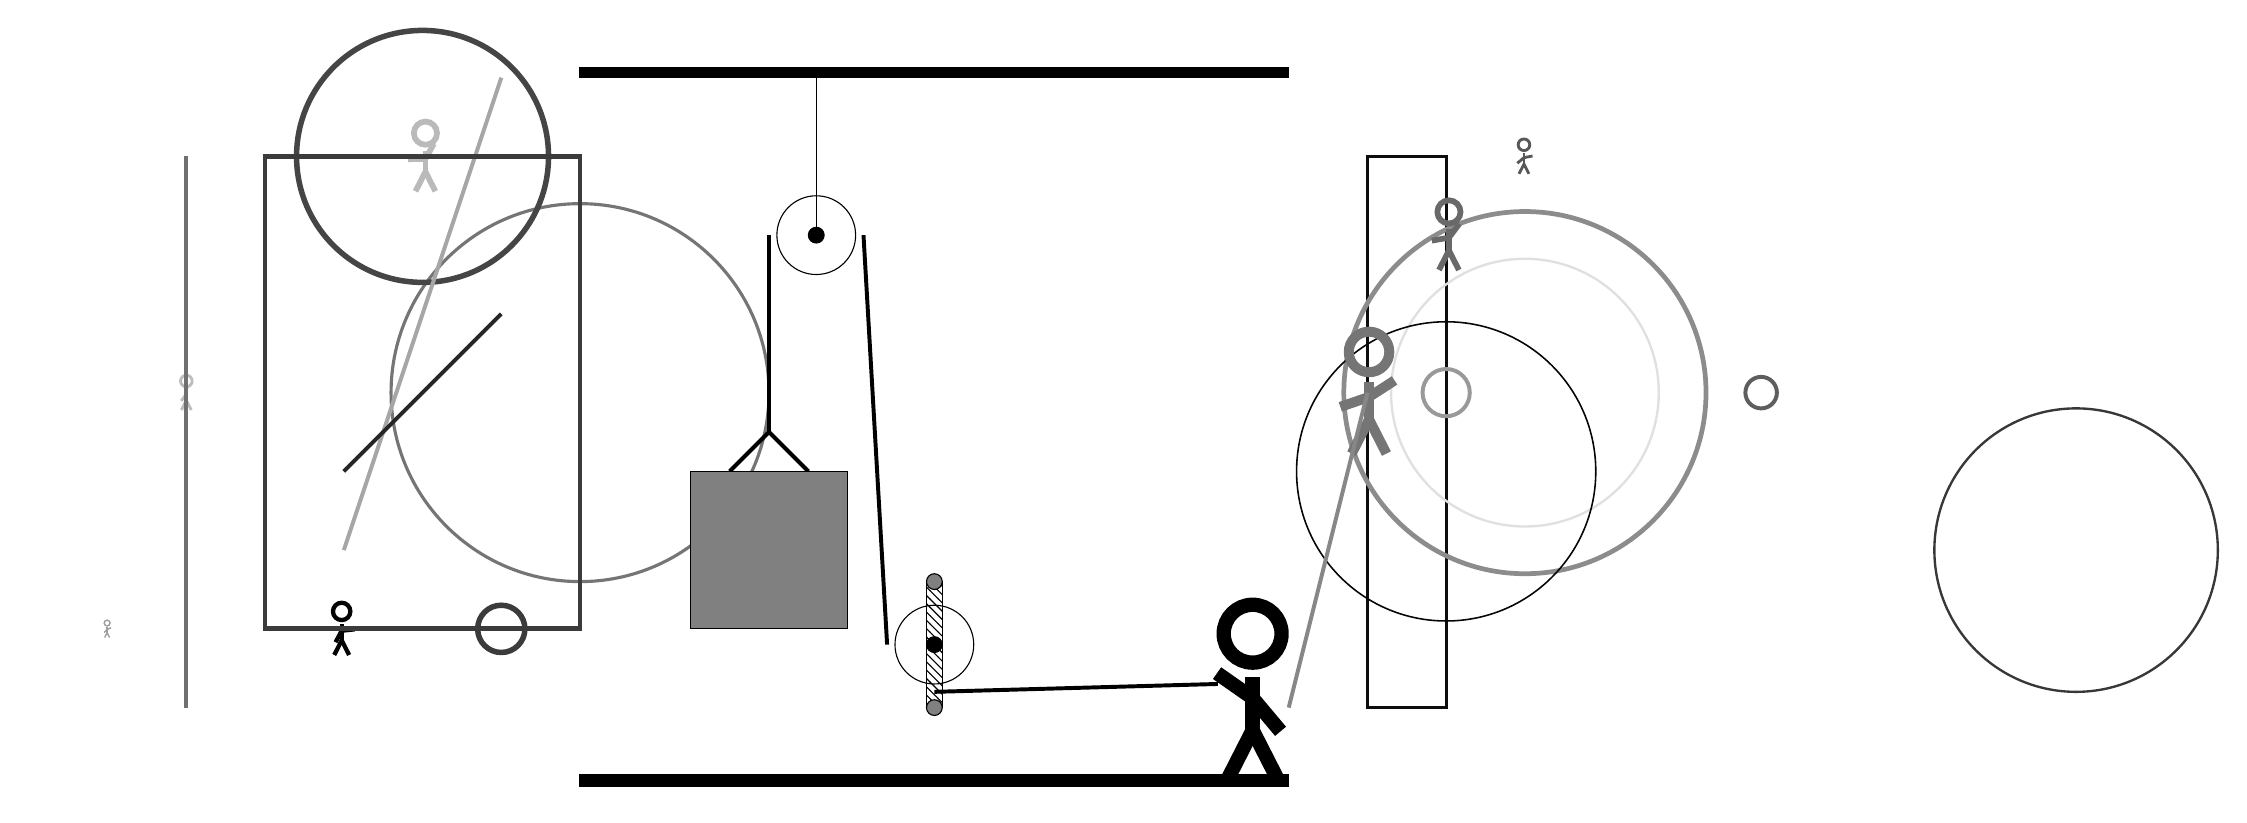
\begin{tikzpicture}
			%%%%% START %%%%%
			
			\draw[fill=black] (-2, 9) rectangle (7, 9.125);
			
			\draw (1, 7) circle (0.5);
			\draw[fill=black] (1, 7) circle (0.1);
			\draw (1, 9) -- (1, 7);
			
			\draw[fill=white](2.5, 1.8) circle (0.5);
			\draw[fill=black] (2.5, 1.8) circle (0.1);
			\draw[pattern=north west lines, pattern color=black] (2.4, 2.6) rectangle (2.6, 1.0);
			\draw[fill=black!50] (2.5, 2.6) circle (0.1);
			\draw[fill=black!50] (2.5, 1.0) circle (0.1);
			
			\node[line width=0.3mm, color=black!27] at (-4, 8) {\Strichmaxerl[4][1][61]};
			
			\node[line width=0.5mm, color=black!26] at (-7, 5) {\Strichmaxerl[2][54][86]};
			\draw [line width=0.3mm, color=black!78](17, 3) circle (1.8);
			\draw [line width=0.4mm, color=black!54](-2, 5) circle (2.4);
			\draw [line width=0.7mm, color=black!73](-4, 8) circle (1.6);
			\draw[line width=0.4mm, color=black!95] (8, 1) rectangle (9, 8);
			\node[line width=0.7mm, color=black!66] at (10, 8) {\Strichmaxerl[2][40][11]};
			\draw[line width=0.5mm, color=black!35](-5, 3) -- (-3, 9);
			\draw [line width=0.3mm, color=black!12](10, 5) circle (1.7);
			\draw [line width=0.6mm, color=black!45](10, 5) circle (2.3);
			\draw[line width=0.5mm, color=black!48](-2, 4) -- (-2, 6);
			\draw [line width=0.5mm, color=black!40](9, 5) circle (0.3);
			\node[line width=0.4mm, color=black!38] at (-8, 2) {\Strichmaxerl[1][46][24]};
			
			\draw [line width=0.5mm, color=black!63](13, 5) circle (0.2);
			\draw[line width=0.5mm, color=black!56](-7, 8) -- (-7, 1);
			\draw[line width=0.5mm, color=black!85](-5, 4) -- (-3, 6);
			\draw [line width=0.2mm, color=black!98](9, 4) circle (1.9);
			\node[line width=0.7mm, color=black!59] at (9, 7) {\Strichmaxerl[4][10][53]};
			\draw [line width=0.7mm, color=black!77](-3, 2) circle (0.3);
			\node[line width=0.7mm, color=black!54] at (8, 5) {\Strichmaxerl[7][19][33]};
			\node[line width=0.5mm, color=black!99] at (-5, 2) {\Strichmaxerl[3][62][6]};
			
			\draw[line width=0.6mm, color=black!77] (-2, 8) rectangle (-6, 2);
			
			\draw [line width=0.3mm, color=black!62](-9, 4) circle (0.0);
			\draw[line width=0.5mm, color=black!47](8, 5) -- (7, 1);
			
			\draw[line width=0.5mm] (-0.1, 4.0) -- (0.4, 4.5) -- (0.9, 4.0);
			\draw[fill=black!50] (-0.6, 4.0) rectangle (1.4, 2.0);
			
			\draw[line width=0.5mm] (0.4, 7) -- (0.4, 4.5);
			\centerarc[line width=0.5mm](1, 7)(0:180:0.6);
			\draw[line width=0.5mm](1.6, 7) -- (1.9, 1.8);
			\centerarc[line width=0.5mm](2.5, 1.8)(180:270:0.6);
			\draw[line width=0.5mm](2.5, 1.2) -- (6.1, 1.3);
			
			\node at (6.5, 1.2) {\Strichmaxerl[10][-35][-50]};
			
			\draw[fill=black] (-2, 0) rectangle (7, 0.15);
			
			%%%%% END %%%%%
		\end{tikzpicture}
	\end{figure}	
\end{document}